
\documentclass[11pt,a4paper]{article}

\usepackage[margin=1in]{geometry}
\usepackage{fontspec}
\setmainfont{Times New Roman}
\setsansfont{Helvetica}
\setmonofont{Menlo}
\usepackage{graphicx}
\usepackage{booktabs}
\usepackage{array}
\usepackage{hyperref}
\usepackage{xcolor}
\usepackage{fancyhdr}
\usepackage{enumitem}
\usepackage{float}
\usepackage{caption}
\usepackage{subcaption}
\usepackage{amsmath,amssymb}
\usepackage{microtype}
\usepackage{setspace}

\hypersetup{
  colorlinks=true,
  linkcolor=blue!50!black,
  urlcolor=blue!60!black,
  pdftitle={Explainable Machine Learning for BTCIRT Limit Order Book Dynamics},
  pdfauthor={Oveys Sayad}
}

\graphicspath{{./}{figures/}}
\setstretch{1.12}
\setlength{\parskip}{0.4em}
\setlength{\parindent}{0pt}
\newcolumntype{L}[1]{>{\raggedright\arraybackslash}p{#1}}

\title{Explainable Machine Learning for BTCIRT\\Limit Order Book Dynamics}
\author{%
  \textbf{Oveys Sayad}\\[0.6em]
  \normalsize
  Email: \href{mailto:oveyssayad@gmail.com}{oveyssayad@gmail.com}\\
  GitHub: \href{https://github.com/OveysSayad}{https://github.com/OveysSayad}\\
  Repository: \href{https://github.com/OveysSayad/explainable-btcirt-lob}{https://github.com/OveysSayad/explainable-btcirt-lob}\\[0.4em]
  \textit{Nobitex $\cdot$ BTCIRT $\cdot$ Sparse LOB Snapshots $\cdot$ Multi-Study Redesign (v2.0)}
}
\date{\today}

\pagestyle{fancy}
\fancyhf{}
\fancyhead[L]{\small Oveys Sayad}
\fancyhead[R]{\small Explainable BTCIRT LOB}
\fancyfoot[C]{\thepage}

\begin{document}
\maketitle
\begin{abstract}
LaTeX report generated from the project README for \texttt{explainable-btcirt-lob}.
Research redesign of explainable ML on sparse Nobitex BTCIRT LOB snapshots
(Studies A/B/C/D), with leakage controls and SHAP explainability figures.
\end{abstract}
\tableofcontents
\newpage


\textbf{Nobitex $\cdot$ BTCIRT $\cdot$ Sparse LOB Snapshots $\cdot$ Multi-Study Redesign (v2.0)}



\begin{quote}
\textbf{Is this a good project to share?} \textbf{Yes --- especially as a research / methodology portfolio piece.} It is strong because it documents \textit{failed designs}, sparse-data honesty, leakage controls, and explainability limits --- not because it claims a trading edge. Share it as \textbf{explainable microstructure ML under realistic data constraints}, not as a profitable bot.
\end{quote}

\vspace{0.5em}

\section{1. Why this project matters}

Most ``LOB $\rightarrow$ next price'' demos quietly assume:


\begin{itemize}
\item dense, regular sampling (e.g. every 100 ms),
\item exact fixed horizons (10s / 30s / 60s),
\item event-level order-flow imbalance (OFI).
\end{itemize}

\textbf{This dataset is not like that.}


Nobitex BTCIRT snapshots arrive with a \textbf{median gap of \textasciitilde{}69 seconds} (development-test median \textasciitilde{}\textbf{189 seconds}). Claiming ``30-second forecasting'' when the next observation is often minutes away is scientifically wrong.


This repository's contribution is therefore:


\begin{center}
\begin{tabular}{L{0.32\linewidth}L{0.58\linewidth}}
\toprule
Contribution & Why it matters \\
\midrule
\textbf{Multi-study redesign} & Separates next-observation, next-change, and strict-horizon questions \\
\textbf{Actual-delay tracking} & Every label stores the real future delay \\
\textbf{Target-timestamp purging} & Prevents label leakage across train/val/test \\
\textbf{Trade deduplication} & Fixes repeated \texttt{last\_trade\_*} inflation \\
\textbf{Explainability triad} & SHAP + permutation + ablation (not SHAP alone) \\
\textbf{Honest failure logs} & Study C underpower \& interaction status logged, not hidden \\
\bottomrule
\end{tabular}
\end{center}
\vspace{0.35em}

\vspace{0.5em}

\section{2. Executive summary of results}

\textbf{Run:} redesign v2.0 $\cdot$ seed \texttt{42} $\cdot$ pipeline completed \textbf{Environment:} Python 3.14 $\cdot$ pandas 3.0.5 $\cdot$ sklearn 1.9 $\cdot$ XGBoost 3.4 $\cdot$ CatBoost 1.2.10 $\cdot$ SHAP 0.52 $\cdot$ macOS arm64


\subsection{Data}

\begin{center}
\begin{tabular}{L{0.32\linewidth}L{0.58\linewidth}}
\toprule
Metric & Value \\
\midrule
Raw rows (all symbols) & \textbf{835,000} \\
BTCIRT retained & \textbf{39,693} (\textbf{4.75\%}) \\
Date range & \textbf{2026-01-04 $\rightarrow$ 2026-02-18} \\
Unique dates & \textbf{44} \\
Median observation gap & \textbf{69.35 s} (test $\approx$ \textbf{188.9 s}) \\
Primary features & \textbf{80} (\texttt{full\_no\_trade}) \\
\bottomrule
\end{tabular}
\end{center}
\vspace{0.35em}

\subsection{Study A --- Next observed mid movement (3-class) --- \textbf{primary}}

\begin{center}
\begin{tabular}{L{0.28\linewidth}L{0.28\linewidth}L{0.28\linewidth}}
\toprule
Model & Development-test Macro F1 & Notes \\
\midrule
Majority & 0.211 & Always STABLE \\
Previous direction & 0.377 &  \\
OBI rule & 0.385 &  \\
\textbf{XGBoost (primary)} & \textbf{0.470} & Frozen specification \\
CatBoost (challenger) & \textbf{0.484} & Competitive; not declared superior without multi-fold proof \\
\bottomrule
\end{tabular}
\end{center}
\vspace{0.35em}

Day-level bootstrap (1000 resamples of dates): Macro F1 mean \textbf{0.470}, 95\% CI \textbf{[0.455, 0.481]}.


Hybrid $\varepsilon$ (train-only) = \textbf{3.664 bps}. Purged sizes: train \textbf{29,568} / val \textbf{5,630} / development\_test \textbf{4,492}.


\subsection{Study B --- Next mid-change direction (binary)}

\begin{center}
\begin{tabular}{L{0.32\linewidth}L{0.58\linewidth}}
\toprule
Item & Value \\
\midrule
Primary samples (1 per price run) & \textbf{25,704} \\
Median time to next change & \textbf{\textasciitilde{}69.6 s} \\
XGBoost Macro F1 (dev-test) & \textbf{0.614} \\
\bottomrule
\end{tabular}
\end{center}
\vspace{0.35em}

\subsection{Study C --- Strict fixed horizons --- \textbf{pilot / underpowered}}

\begin{center}
\begin{tabular}{L{0.22\linewidth}L{0.22\linewidth}L{0.22\linewidth}L{0.22\linewidth}}
\toprule
Horizon & Window & Eligible & Modeling \\
\midrule
10 s & [5, 15] & \textbf{0} & Underpowered pilot \\
30 s & [20, 40] & \textbf{0} & Underpowered pilot \\
60 s & [40, 80] & \textbf{29,318} & Eligible overall, but \textbf{0} development\_test rows after target purge $\rightarrow$ \textbf{no robust claim} \\
\bottomrule
\end{tabular}
\end{center}
\vspace{0.35em}

\subsection{Incremental value (development\_test Macro F1)}

\begin{center}
\begin{tabular}{L{0.32\linewidth}L{0.58\linewidth}}
\toprule
Quantity & Δ Macro F1 \\
\midrule
LOB vs price-only (\texttt{full\_no\_trade - price\_only}) & \textbf{+0.046} \\
Corrected trades (\texttt{full\_with\_trade - full\_no\_trade}) & \textbf{-0.001} \\
Time features (\texttt{full\_no\_trade - full\_no\_time}) & \textbf{+0.004} \\
\bottomrule
\end{tabular}
\end{center}
\vspace{0.35em}

\textbf{Interpretation:} LOB state adds measurable lift over returns/volatility alone. Corrected trade intensity does \textbf{not} help. Time features add a tiny lift and must be audited for collection artifacts.


\vspace{0.5em}

\section{3. Research questions}

\subsection{Study A --- Next observed mid-price movement}

\begin{quote}
Can the current and recent LOB state predict whether the \textbf{next observed} mid-price moves \textbf{DOWN / STABLE / UP}?
\end{quote}

Uses consecutive snapshots. Stores \texttt{actual\_delay\_seconds}. Does \textbf{not} claim an exact clock horizon.


\subsection{Study B --- Next mid-price \textit{change} direction}

\begin{quote}
Conditional on the mid eventually changing, can the book predict \textbf{UP vs DOWN}?
\end{quote}

Skips unchanged mids; primary sample = one observation per flat price-run.


\subsection{Study C --- Strict 10 / 30 / 60 second forecasting}

\begin{quote}
On samples whose future observation delay truly falls in a narrow window, is fixed-horizon prediction feasible?
\end{quote}

Defaults: 10∈[5,15], 30∈[20,40], 60∈[40,80]. Under sparse sampling this is mostly a \textbf{pilot}.


\subsection{Study D --- Dense data-collection design}

Documentation only (\texttt{docs/DENSE\_DATA\_COLLECTION\_DESIGN.md}). No fabricated WebSocket data.


\vspace{0.5em}

\section{4. End-to-end project flow}

\begin{verbatim}
raw CSV
  │
  ▼
[1] data_loader.py          filter exchange=nobitex, symbol=BTCIRT (normalized)
  │
  ▼
[2] data_validation.py      crossed books, ordering, missing/inf, duplicates
  │
  ▼
[3] preprocessing.py        keep-last duplicate timestamps; NO 5s grid
  │
  ▼
[4] delay_audit.py          gap histograms & percentiles (overall / date / hour / split)
  │
  ▼
[5] feature_engineering.py  stationary LOB + lags + snapshot OFI proxies + optional trades
  │
  ▼
[6] labels/
      next_observation.py   Study A
      next_price_change.py  Study B
      strict_horizon.py     Study C + horizon overlap
  │
  ▼
[7] splitting/              date split + target-timestamp purge + walk-forward folds
  │
  ▼
[8] models/                 baselines → logistic → XGBoost → CatBoost
  │
  ▼
[9] evaluation/             metrics + day bootstrap + financial sanity (exploratory)
  │
  ▼
[10] explainability/        SHAP + permutation + ablation + interaction fallbacks
  │
  ▼
[11] reporting              tables / figures / frozen spec / reports/final_report.md
\end{verbatim}

\textbf{One command for the full path:}


\begin{verbatim}
./scripts/run_pipeline.sh
# equivalent:
python -m src.pipeline --config configs/project_config.yaml
\end{verbatim}

\vspace{0.5em}

\section{5. Repository map \& code logic}

\begin{verbatim}
explainable-btcirt-lob/
├── configs/                 YAML: project + per-study overrides
├── src/
│   ├── pipeline.py          Orchestrator (Studies A/B/C)
│   ├── data_loader.py       Chunked CSV load + BTCIRT filter
│   ├── data_validation.py   Book integrity audits
│   ├── preprocessing.py     Cleaning; refuses dense grid when gaps are large
│   ├── delay_audit.py       Observation-gap statistics
│   ├── feature_engineering.py
│   ├── trade_deduplication.py
│   ├── labels/              Study A / B / C label builders
│   ├── splitting/           Chronological + purge + walk-forward
│   ├── models/              Baselines, logistic, XGB, CatBoost, calibration, two-stage
│   ├── evaluation/          Metrics, bootstrap, financial sanity
│   ├── explainability/      SHAP, grouped SHAP, permutation, ablation, interactions
│   ├── visualization.py     Figures
│   └── reporting.py         Report helpers (run summaries → reports/)
├── docs/                    Design, formulas, validation, limitations
├── tests/                   46 unit tests (units, labels, purge, no-leakage)
├── scripts/                 run_pipeline / study_a|b|c / tests
├── reports/
│   ├── archive/pre_research_redesign/   frozen v1 outputs
│   ├── tables/              CSV results
│   ├── metrics/             JSON metrics
│   ├── figures/             PNG figures
│   ├── models/              frozen_model_specification.json
│   └── final_report.md
└── notebooks/               Thin wrappers that import from src/
\end{verbatim}

\subsection{Logic highlights by module}

\begin{center}
\begin{tabular}{L{0.32\linewidth}L{0.58\linewidth}}
\toprule
Module & Core logic \\
\midrule
\texttt{data\_loader} & Normalize \texttt{exchange.lower()}, \texttt{symbol.upper()}; keep only \texttt{nobitex} + \texttt{BTCIRT}; raise if empty \\
\texttt{preprocessing} & Sort time; keep \textbf{last} duplicate timestamp; skip 5s alignment when median gap ≫ 5s \\
\texttt{labels/next\_observation} & \texttt{target = t+1}; return in bps; hybrid $\varepsilon$ from \textbf{train only} \\
\texttt{labels/next\_price\_change} & Forward scan to first mid $\ne$ current; optional one-sample-per-run \\
\texttt{labels/strict\_horizon} & Match only inside \texttt{[lower, upper]}; minimize ` \\
\texttt{splitting/purged\_split} & Drop rows whose \texttt{target\_timestamp} crosses the next split boundary \\
\texttt{trade\_deduplication} & Signature \texttt{(price, qty)} $\rightarrow$ \texttt{is\_new\_trade}; repeated snapshots count as 0 \\
\texttt{feature\_engineering} & Depth / OBI / WOBI / microprice / snapshot OFI proxy / 120--1200s windows / event lags \\
\texttt{models/xgboost\_model} & Randomized search on \textbf{validation Macro F1}; never on development\_test \\
\texttt{explainability/*} & TreeSHAP; on interaction failure $\rightarrow$ dependence fallbacks + JSON status \\
\bottomrule
\end{tabular}
\end{center}
\vspace{0.35em}

Notebooks \textbf{must not} re-implement formulas; they import \texttt{src/}.


\vspace{0.5em}

\section{6. Dataset \& filtering}

\begin{itemize}
\item \textbf{File:} \texttt{data/raw/market\_data\_clean\_nobitex.csv} (\textbf{not committed} --- place locally)
\item \textbf{Exchange / symbol:} \texttt{nobitex} / \texttt{BTCIRT}
\item \textbf{LOB:} 8 ask + 8 bid price/qty levels
\item \textbf{Trades:} \texttt{last\_trade\_price}, \texttt{last\_trade\_qty} (often repeated across snapshots)
\item \textbf{JSON columns} (\texttt{data}, \texttt{asks}, \texttt{bids}, \texttt{last\_trade}): unused when flattened columns exist
\end{itemize}

\begin{verbatim}
df["exchange"] = df["exchange"].astype(str).str.strip().str.lower()
df["symbol"] = df["symbol"].astype(str).str.strip().str.upper()
df = df[(df["exchange"] == "nobitex") & (df["symbol"] == "BTCIRT")]
\end{verbatim}

\vspace{0.5em}

\section{7. Data-quality \& observation-gap audit}

\subsection{Quality checks}

Missing / infinite values $\cdot$ zero/negative prices \& quantities $\cdot$ crossed books (\texttt{a1 $\le$ b1}) $\cdot$ locked books $\cdot$ invalid ask/bid monotonicity $\cdot$ abnormal spreads $\cdot$ timestamp parse failures $\cdot$ exact \& timestamp duplicates.


\subsection{Gap reality (this run)}

\begin{center}
\begin{tabular}{L{0.22\linewidth}L{0.22\linewidth}L{0.22\linewidth}L{0.22\linewidth}}
\toprule
Segment & Median gap (s) & \% gaps > 60s & \% gaps > 120s \\
\midrule
Overall & \textbf{69.35} & \textbf{100\%} & 18.9\% \\
Train & 68.88 & 100\% & 1.6\% \\
Validation & 71.10 & 100\% & 45.3\% \\
Development test & \textbf{188.88} & 100\% & \textbf{100\%} \\
\bottomrule
\end{tabular}
\end{center}
\vspace{0.35em}

\textbf{Consequence:} every gap exceeds 10s and 30s $\rightarrow$ Study C 10s/30s eligibility = \textbf{0}. A 60s window (40--80s) matches many train/val snapshots whose next print is \textasciitilde{}70s, but the late-period test gaps (\textasciitilde{}3 minutes) fall \textbf{outside} the 80s upper bound after purging.


Tables: \texttt{reports/tables/observation\_gap\_summary.csv}, \texttt{observation\_gap\_by\_date.csv}, \texttt{observation\_gap\_by\_hour.csv}.


\subsection{Visual evidence}

\begin{figure}[H]
\centering
\begin{subfigure}[t]{0.47\linewidth}
\centering
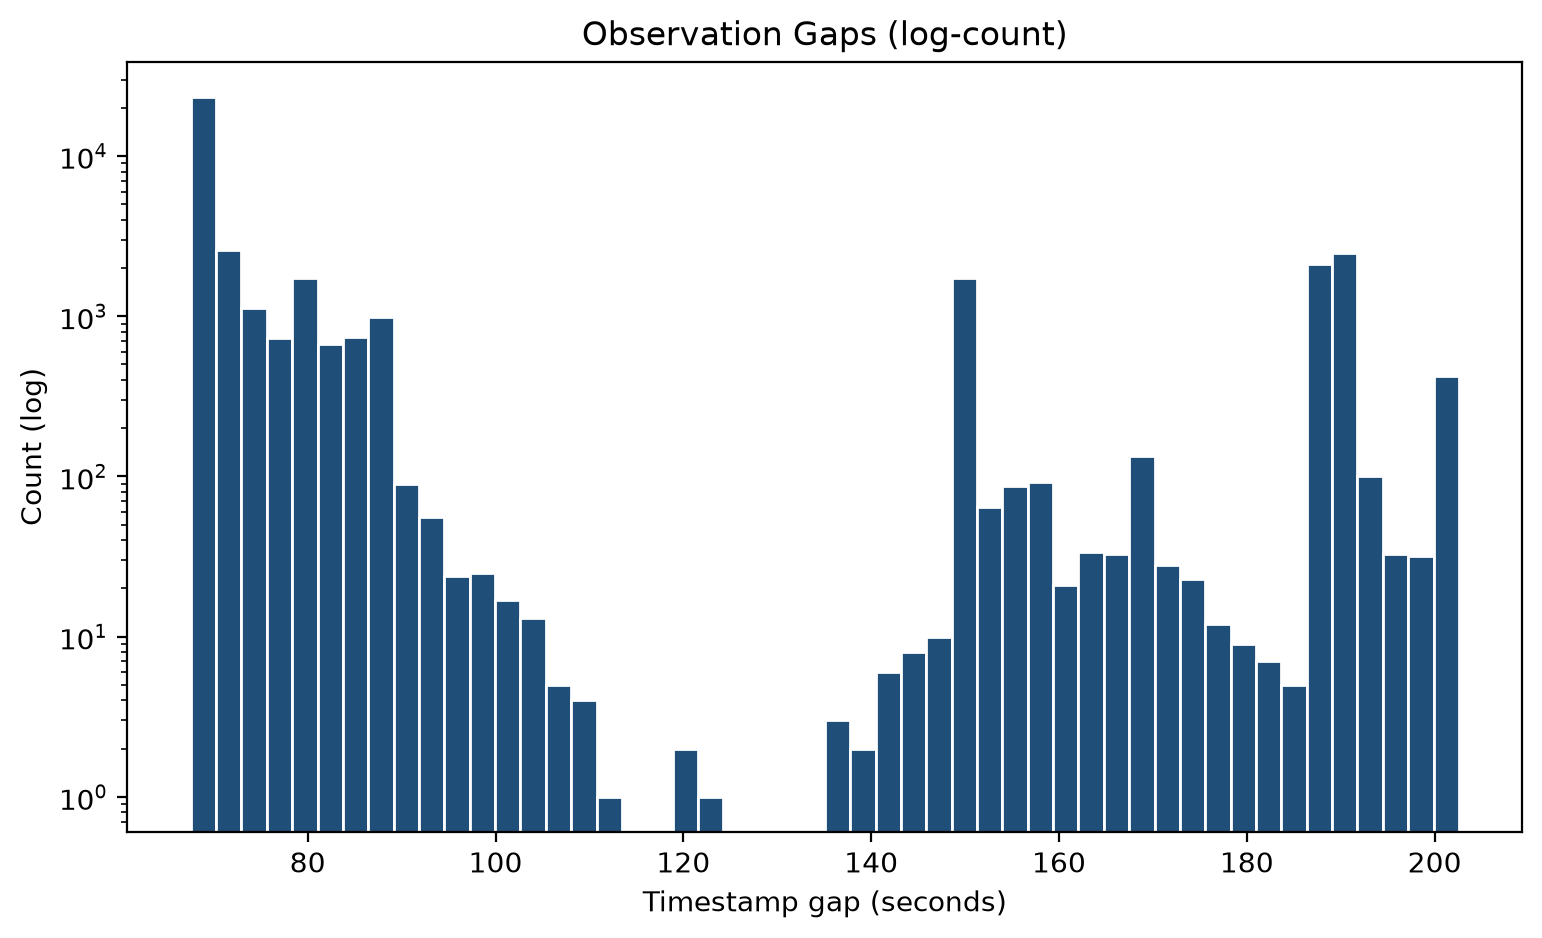
\includegraphics[width=\linewidth]{figures/data_quality/observation_gap_hist_log.png}
\caption*{Observation gaps (log scale)}
\end{subfigure}
\hfill
\begin{subfigure}[t]{0.47\linewidth}
\centering
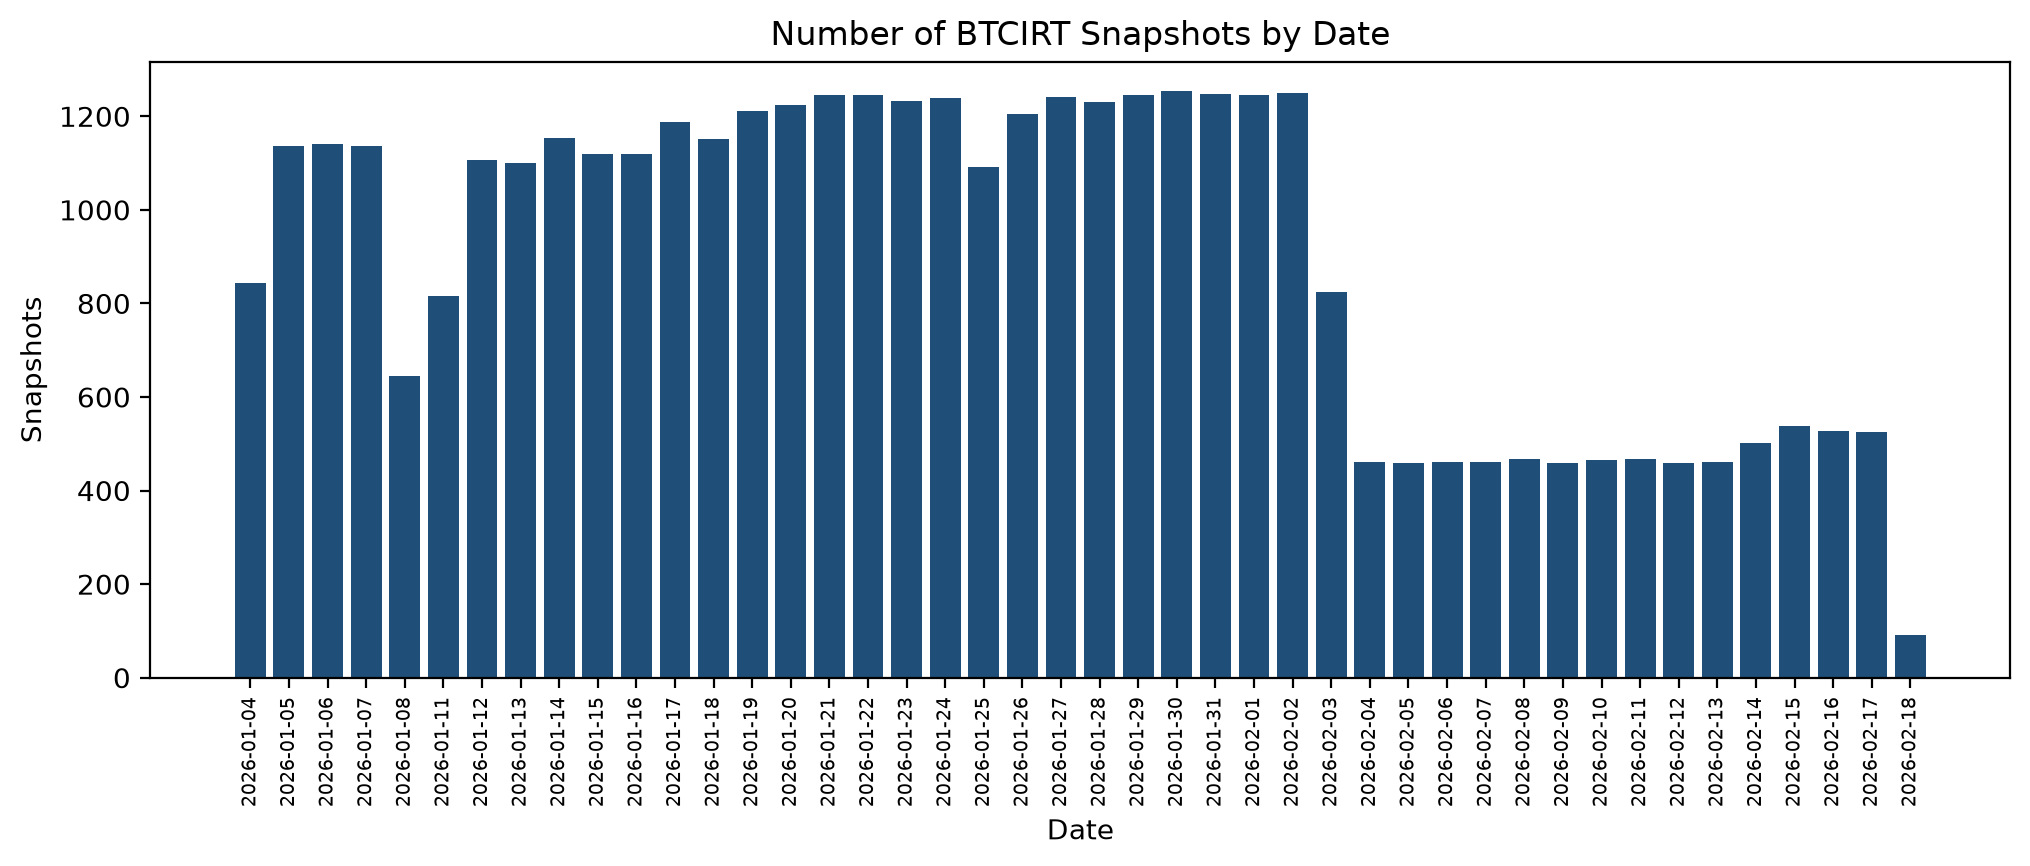
\includegraphics[width=\linewidth]{figures/data_quality/snapshots_by_date.png}
\caption*{Snapshots by date}
\end{subfigure}
\end{figure}

\begin{figure}[H]
\centering
\begin{subfigure}[t]{0.47\linewidth}
\centering
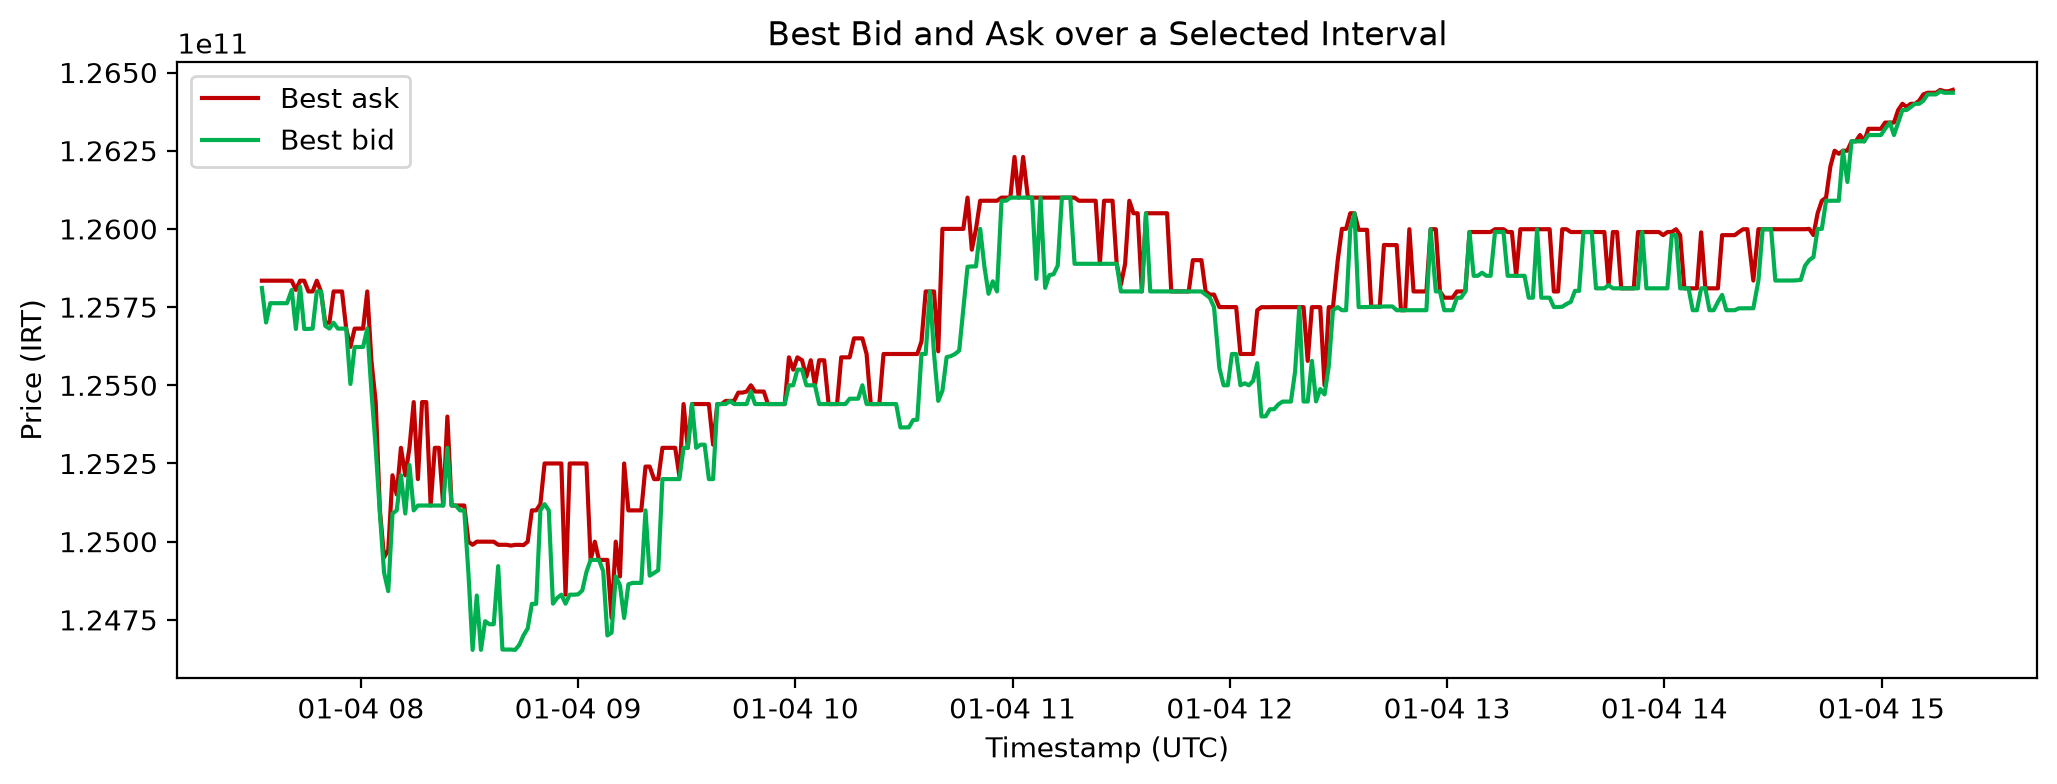
\includegraphics[width=\linewidth]{figures/data_quality/best_bid_ask_window.png}
\caption*{Best bid / ask window}
\end{subfigure}
\hfill
\begin{subfigure}[t]{0.47\linewidth}
\centering
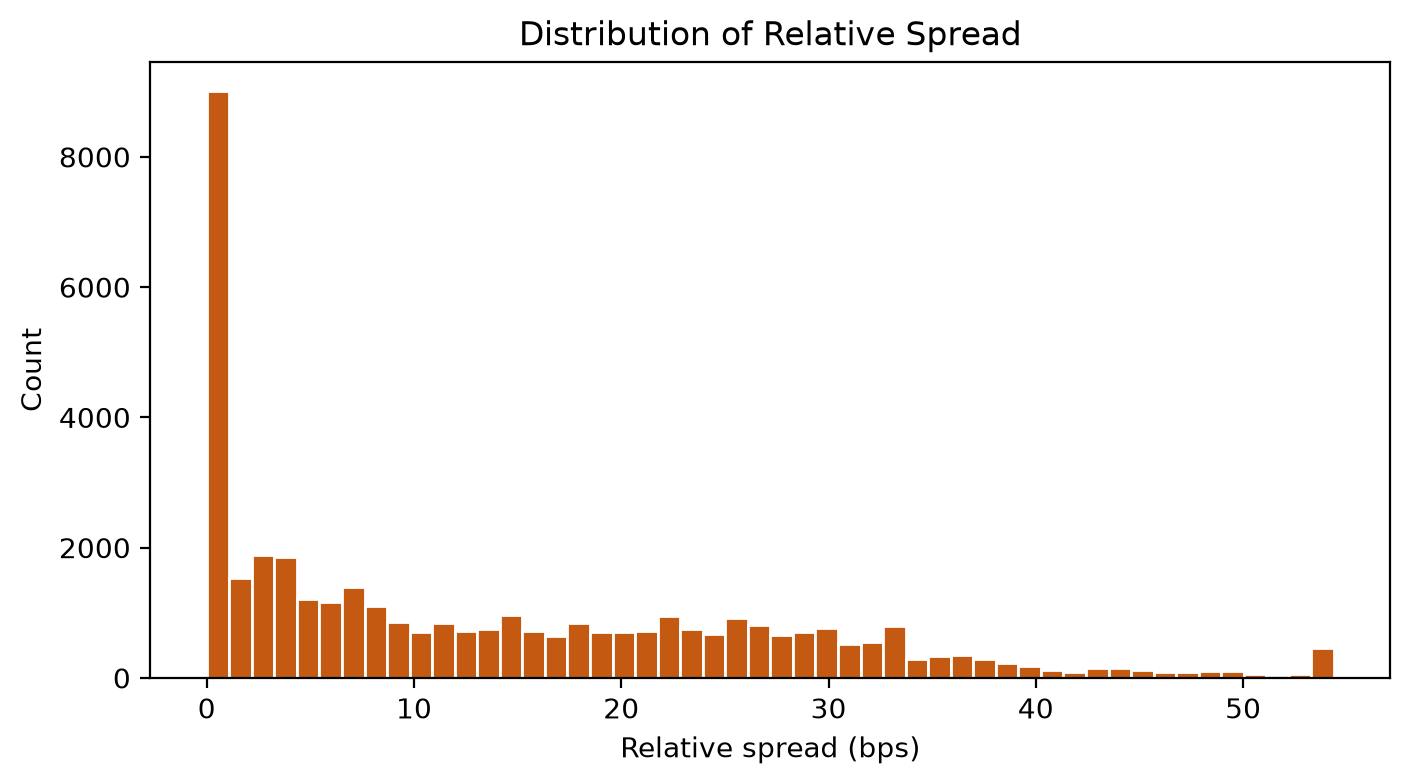
\includegraphics[width=\linewidth]{figures/data_quality/relative_spread_distribution.png}
\caption*{Relative spread distribution}
\end{subfigure}
\end{figure}

\begin{figure}[H]
\centering
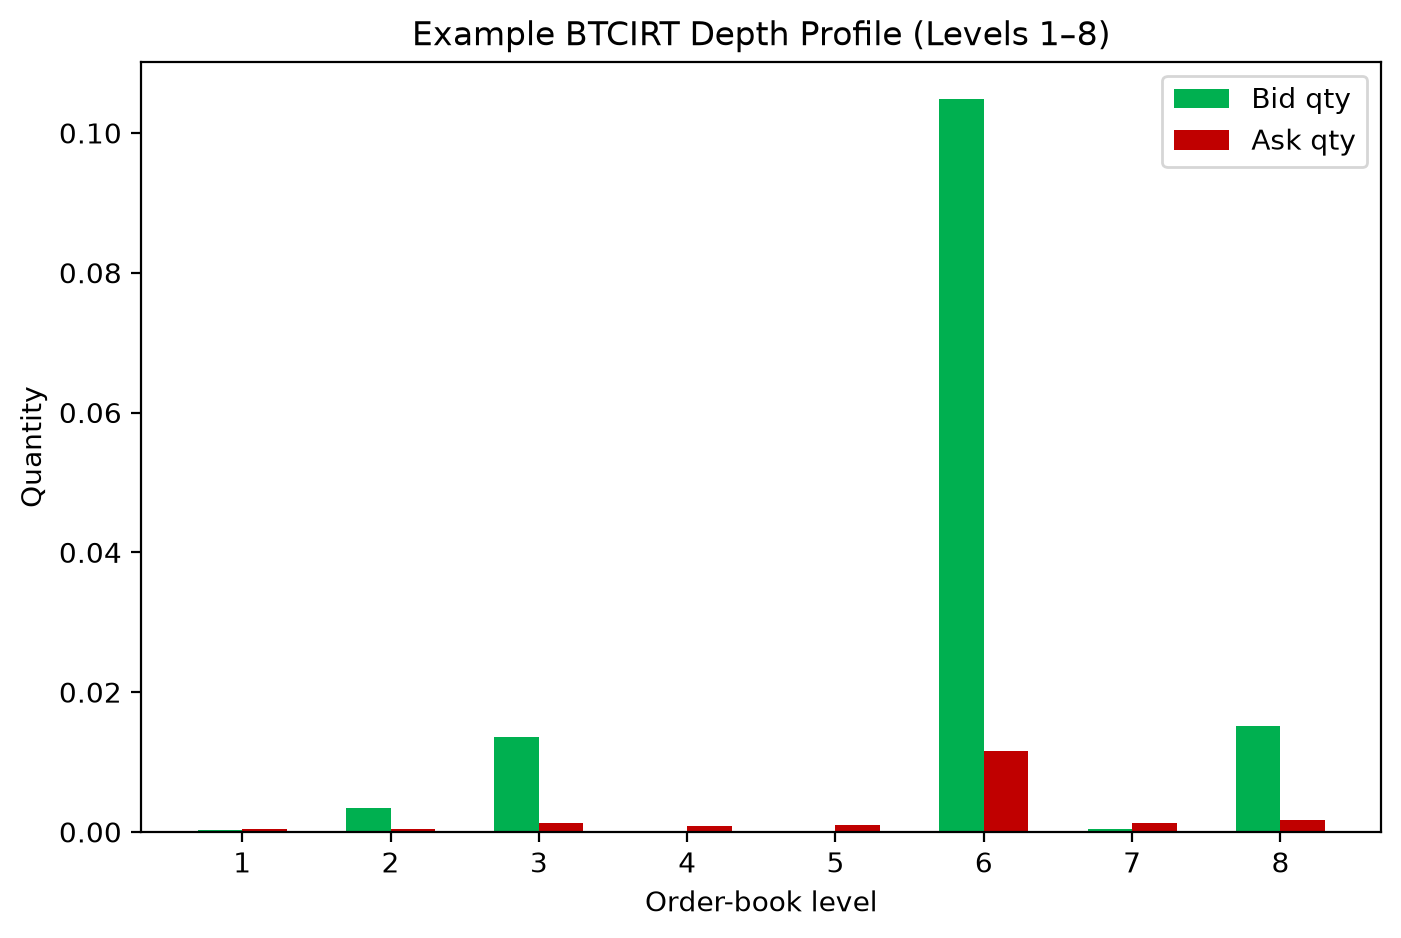
\includegraphics[width=0.70\linewidth]{figures/data_quality/depth_profile_example.png}
\caption{LOB depth profile example}
\end{figure}

\begin{center}\textit{Example depth profile --- liquidity is concentrated near the touch.}\end{center}

\vspace{0.5em}

\section{8. Mathematical core}

Formulas use GitHub-flavored LaTeX (\texttt{\$$ ... $\$}). Full catalog: \href{docs/FORMULAS.md}{\texttt{docs/FORMULAS.md}}.


\subsection{Mid-price, spread, relative spread}

\[
m_t = \frac{a_{1,t} + b_{1,t}}{2}, \qquad
S_t = a_{1,t} - b_{1,t}, \qquad
\mathrm{RelSpreadBps}_t = 10^{4}\,\frac{S_t}{m_t}
\]

\subsection{Log return in basis points}

Unit-tested so $10^{4}\log(100.01/100)\approx 1$:


\[
r = 10^{4}\,\log\left(\frac{m_{\mathrm{future}}}{m_{\mathrm{current}}}\right)
\]

\subsection{Order-book imbalance (depth $k$)}

\[
D^{a}_{k,t}=\sum_{i=1}^{k} q^{a}_{i,t}, \qquad
D^{b}_{k,t}=\sum_{i=1}^{k} q^{b}_{i,t}
\]

\[
\mathrm{OBI}_{k,t}=\frac{D^{b}_{k,t}-D^{a}_{k,t}}{D^{b}_{k,t}+D^{a}_{k,t}+\delta}
\]

where $\delta$ is a tiny constant for numerical stability (e.g. $10^{-12}$).


\subsection{Weighted OBI}

Weights $w_i=e^{-\lambda(i-1)}$ with default $\lambda=0.5$:


\[
\mathrm{WOBI}_t=
\frac{\sum_{i} w_i q^{b}_{i,t}-\sum_{i} w_i q^{a}_{i,t}}
{\sum_{i} w_i q^{b}_{i,t}+\sum_{i} w_i q^{a}_{i,t}+\delta}
\]

\subsection{Snapshot OFI proxy (not event-level OFI)}

\[
e^{b}_{t}=
\mathbf{1}_{\{b_t \ge b_{t-1}\}}\,q^{b}_{t}
-
\mathbf{1}_{\{b_t \le b_{t-1}\}}\,q^{b}_{t-1}
\]

(and similarly for the ask side with opposite inequalities)


\[
\mathrm{OFIProxy}_t = e^{b}_{t} - e^{a}_{t}
\]

\subsection{Tick size}

Empirical mode of positive quote diffs = \textbf{10 IRT}. In bps vs huge BTCIRT mids this is $\sim 10^{-6}$ bps, so hybrid $\varepsilon$ relies on return quantiles / spreads, not ticks.


\vspace{0.5em}

\section{9. Label construction}

\subsection{Study A}

Next snapshot return $\rightarrow$ classes with train-only hybrid $\varepsilon$:


\[
\varepsilon=
\max
\bigl(
\varepsilon_{Q},\;
\varepsilon_{\mathrm{tick}},\;
0.5\times \mathrm{MedianSpreadBps}_{\mathrm{train}}
\bigr)
\]

\[
y_t=
\begin{cases}
\mathrm{DOWN} & \text{if } r_t < -\varepsilon \\[4pt]
\mathrm{STABLE} & \text{if } |r_t| \le \varepsilon \\[4pt]
\mathrm{UP} & \text{if } r_t > \varepsilon
\end{cases}
\]

\textbf{This run:} $\varepsilon = 3.664$ bps $\cdot$ method = \texttt{hybrid} $\cdot$ median delay $\approx 69.35$ s.


\textbf{Class mix (development\_test):} DOWN \textbf{27.3\%} $\cdot$ STABLE \textbf{46.3\%} $\cdot$ UP \textbf{26.4\%}.


\begin{figure}[H]
\centering
\begin{subfigure}[t]{0.47\linewidth}
\centering
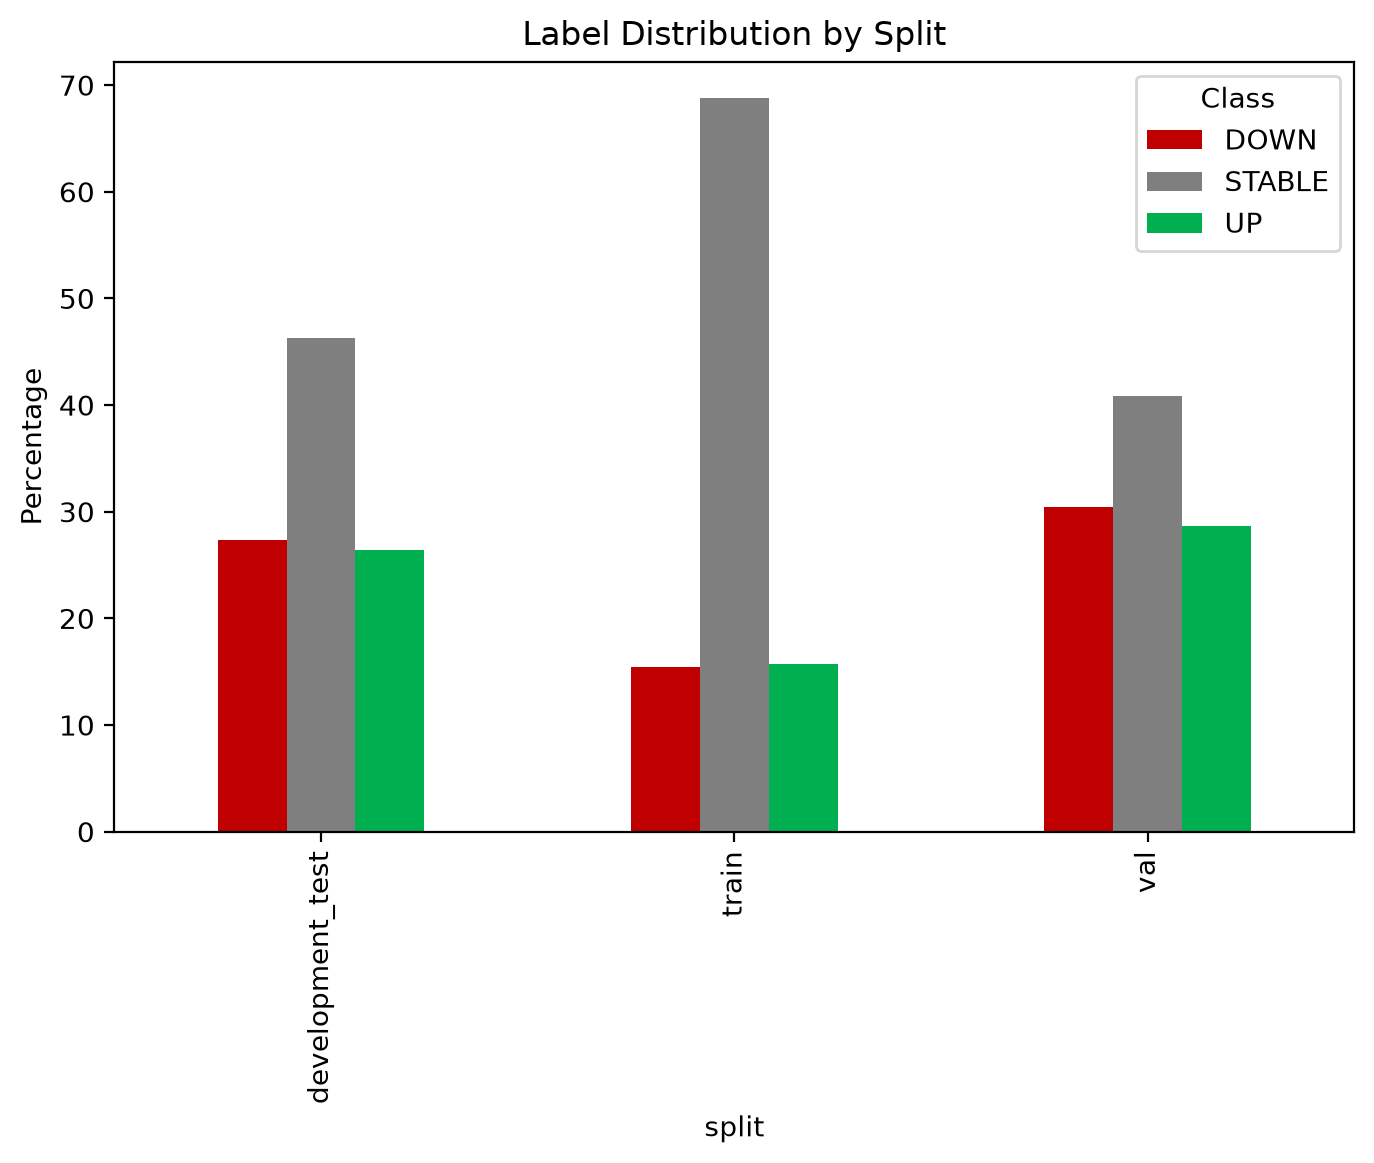
\includegraphics[width=\linewidth]{figures/labels/study_a_class_distribution.png}
\caption*{Study A class mix by split}
\end{subfigure}
\hfill
\begin{subfigure}[t]{0.47\linewidth}
\centering
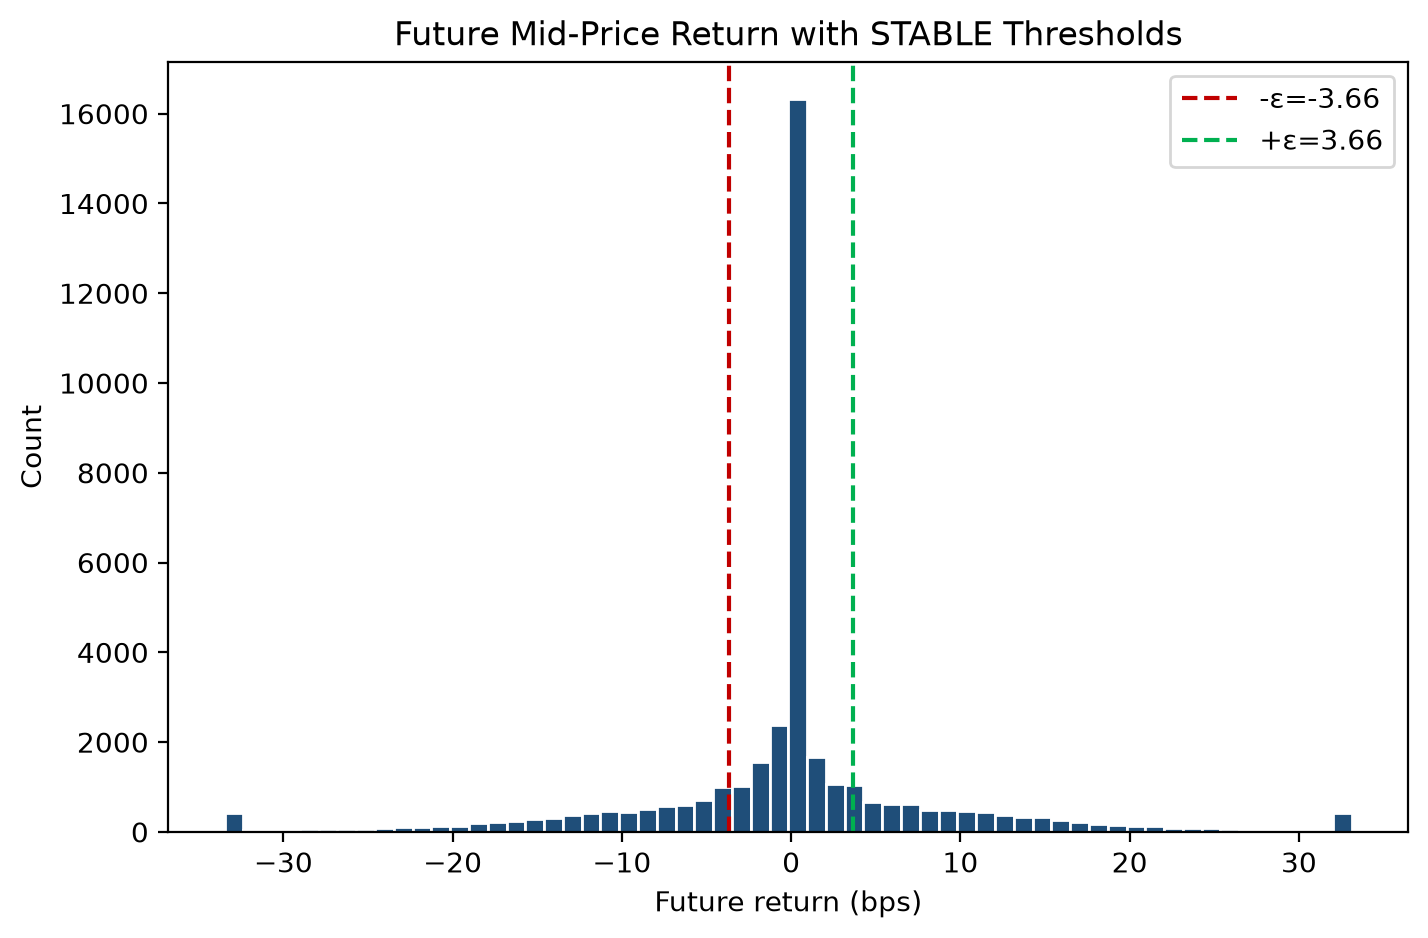
\includegraphics[width=\linewidth]{figures/labels/next_observation_return_epsilon.png}
\caption*{Next-observation returns vs $\varepsilon$}
\end{subfigure}
\end{figure}

\begin{figure}[H]
\centering
\begin{subfigure}[t]{0.47\linewidth}
\centering
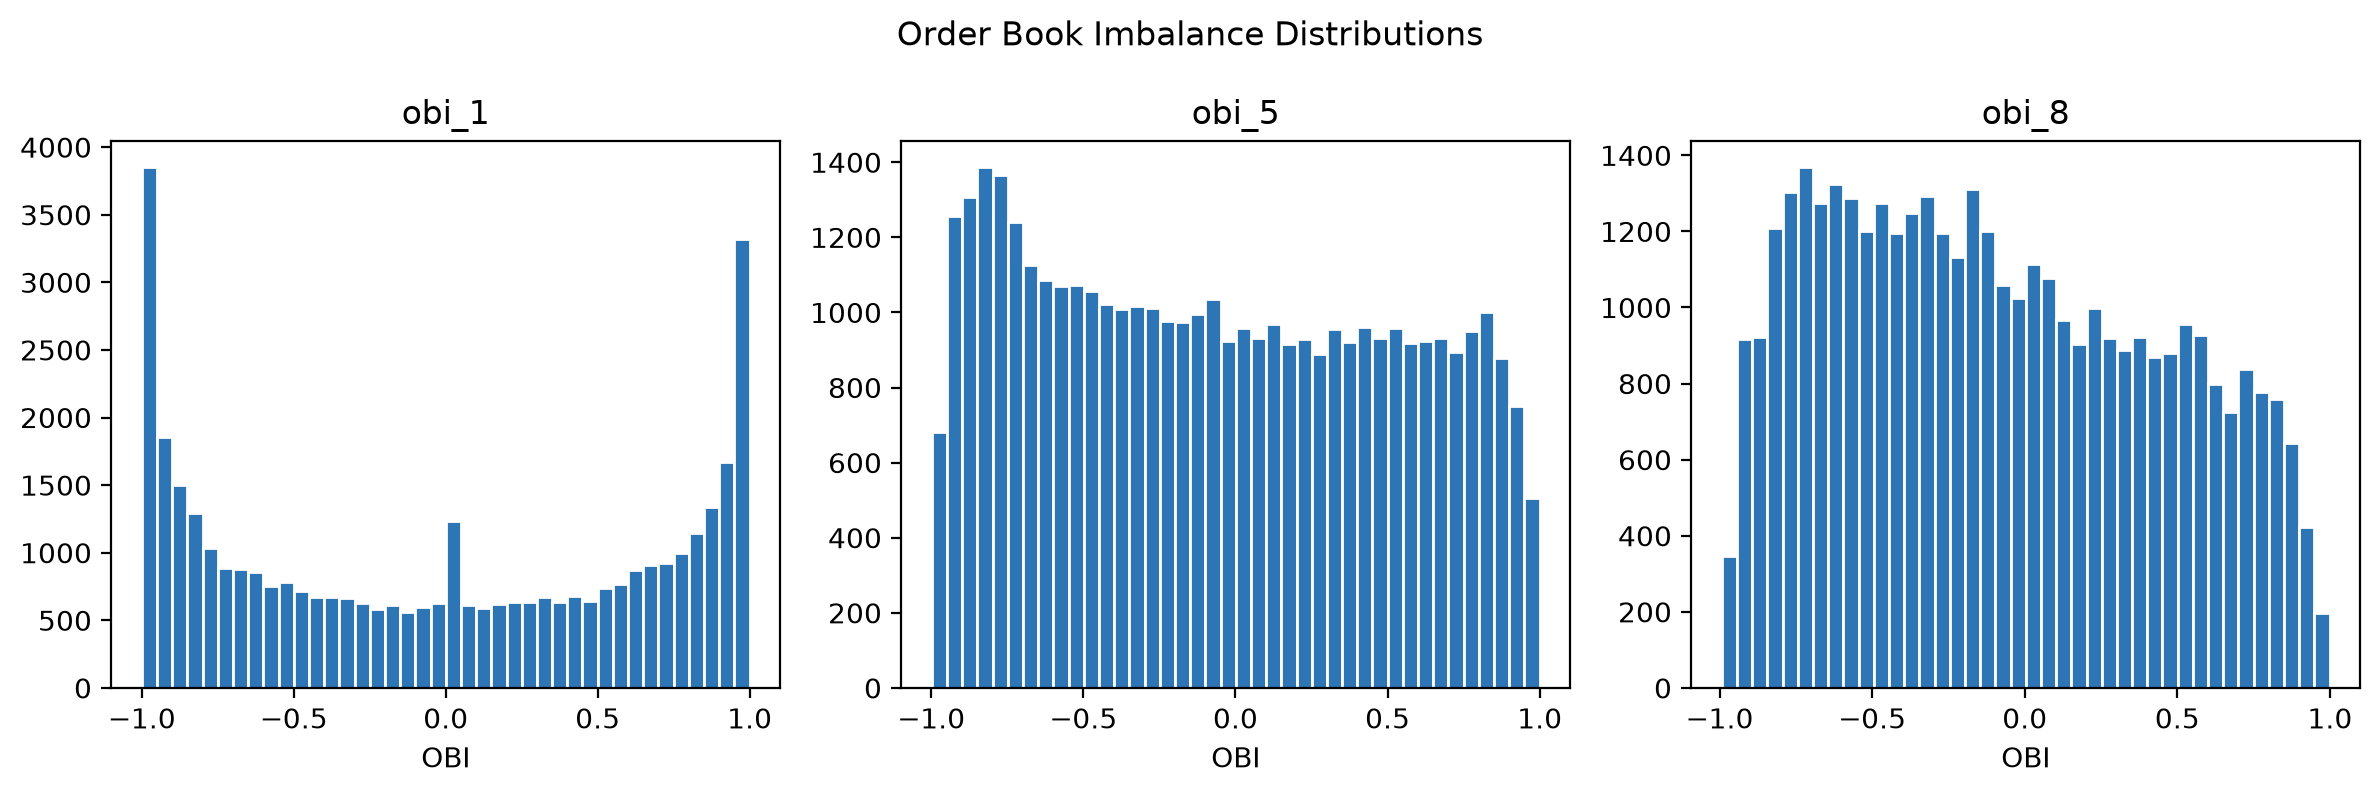
\includegraphics[width=\linewidth]{figures/labels/obi_distributions.png}
\caption*{OBI distributions}
\end{subfigure}
\hfill
\begin{subfigure}[t]{0.47\linewidth}
\centering
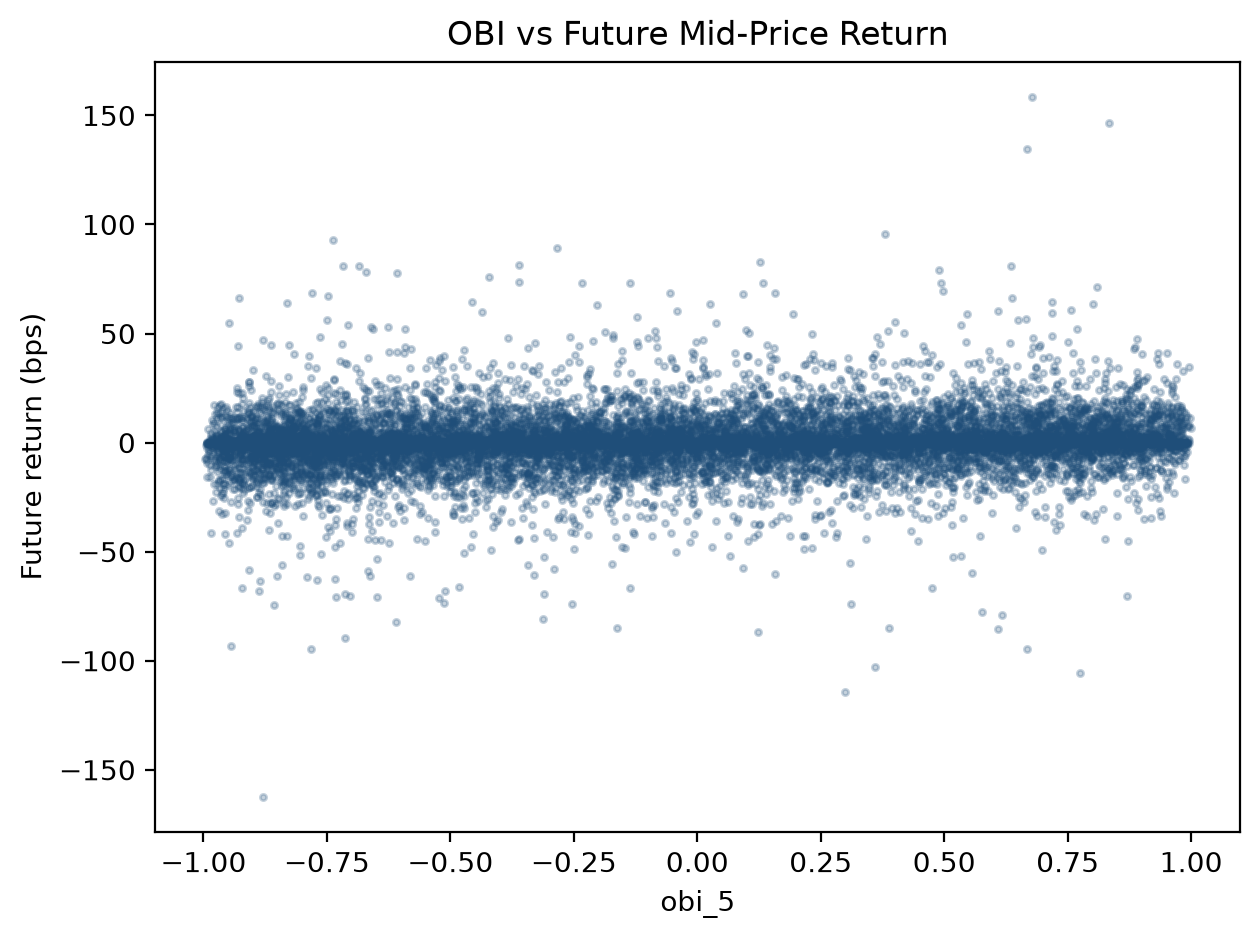
\includegraphics[width=\linewidth]{figures/labels/obi_vs_next_return.png}
\caption*{OBI vs next return}
\end{subfigure}
\end{figure}

\subsection{Study B}

First future mid $\neq$ current $\rightarrow$ UP / DOWN. Primary sample = last snapshot of each unchanged price run (avoids flooding one future event).


\subsection{Study C}

Keep a future snapshot $s$ only when the delay is inside the strict window:


\[
\mathrm{Lower}_h \le t_s - t_t \le \mathrm{Upper}_h
\]

Defaults: $10\mathrm{s}\rightarrow[5,15]$, $30\mathrm{s}\rightarrow[20,40]$, $60\mathrm{s}\rightarrow[40,80]$. Among matches, minimize $|t_s-t_t-h|$. Store \texttt{actual\_delay\_seconds} and \texttt{horizon\_error\_seconds}.


\vspace{0.5em}

\section{10. Feature engineering}

\subsection{Families}

Price history $\cdot$ Static liquidity / depth / imbalance $\cdot$ Dynamic liquidity / imbalance $\cdot$ Snapshot OFI proxy $\cdot$ Volatility $\cdot$ Trade activity (corrected) $\cdot$ Time $\cdot$ Data-collection metadata (\texttt{observation\_gap\_seconds}, \textbf{excluded} from primary).


\subsection{Mandatory feature sets}

\begin{center}
\begin{tabular}{L{0.32\linewidth}L{0.58\linewidth}}
\toprule
Set & Contents \\
\midrule
\texttt{price\_only} & Returns + volatility \\
\texttt{static\_lob} / \texttt{dynamic\_lob} / \texttt{lob\_full} & Book structure \& dynamics \\
\textbf{\texttt{full\_no\_trade}} & Primary model \\
\texttt{full\_with\_trade} & + corrected trades \\
\texttt{full\_no\_time} & Drop cyclical hour/dow \\
\bottomrule
\end{tabular}
\end{center}
\vspace{0.35em}

Dictionary: \texttt{reports/tables/feature\_dictionary.csv} $\cdot$ \texttt{docs/FEATURE\_DICTIONARY.md}.


\vspace{0.5em}

\section{11. Temporal validation \& leakage control}

\begin{enumerate}
\item Split by \textbf{complete calendar dates} (60\% / 20\% / 20\%).
\item Latest block = \textbf{\texttt{development\_test}} --- already inspected in prior analysis $\rightarrow$ \textbf{not a pristine holdout}.
\item \textbf{Target-timestamp purging:} a training row is kept only if \texttt{target\_timestamp < validation\_start} (same idea for val vs test).
\item Scalers, $\varepsilon$, class weights, and hyperparameter search fit on \textbf{training / validation only}.
\item Frozen spec written to \texttt{reports/models/frozen\_model\_specification.json}.
\item \textbf{Final independent future holdout ($\ge$7--14 new days) is still pending.}
\end{enumerate}

Tests: \texttt{tests/test\_purging.py}, \texttt{tests/test\_no\_leakage.py}.


\vspace{0.5em}

\section{12. Models \& hyperparameters}

\subsection{Baselines}

Majority $\cdot$ stratified random $\cdot$ previous mid-direction $\cdot$ OBI-5 threshold rule (tuned on train).


\subsection{Primary: XGBoost}

\begin{itemize}
\item Study A: \texttt{multi:softprob} (3-class)
\item Study B: \texttt{binary:logistic}
\item Search objective: \textbf{validation Macro F1}
\item Early stopping on validation
\item CPU \texttt{tree\_method=hist}
\end{itemize}

\textbf{Best Study A params (this run):}


\begin{verbatim}
max_depth=7, learning_rate=0.02, n_estimators=1500,
min_child_weight=3, subsample=0.8, colsample_bytree=0.8,
gamma=0, reg_alpha=1, reg_lambda=5, max_delta_step=5,
random_state=42
\end{verbatim}

\textbf{Best Study B params:}


\begin{verbatim}
max_depth=6, learning_rate=0.02, n_estimators=500,
min_child_weight=5, subsample=0.8, colsample_bytree=0.5,
gamma=1, reg_alpha=0.1, reg_lambda=20, max_delta_step=5
\end{verbatim}

\subsection{Challenger: CatBoost}

Study A best (this run): \texttt{depth=7}, \texttt{learning\_rate=0.1}, \texttt{iterations=750}, \texttt{l2\_leaf\_reg=10}, \texttt{border\_count=64}, \texttt{subsample=1.0} (Bernoulli bootstrap; \texttt{bagging\_temperature} removed --- incompatible with Bernoulli).


Details: \href{docs/MODEL_SPECIFICATION.md}{\texttt{docs/MODEL\_SPECIFICATION.md}}.


\vspace{0.5em}

\section{13. Full results (this run)}

\subsection{Study A --- model comparison (development\_test)}

\begin{center}
\begin{tabular}{L{0.16\linewidth}L{0.16\linewidth}L{0.16\linewidth}L{0.16\linewidth}L{0.16\linewidth}}
\toprule
Model & Macro F1 & Balanced Acc & Log Loss & MCC \\
\midrule
Majority & 0.211 & 0.333 & --- & 0.000 \\
Previous direction & 0.377 & 0.377 & --- & 0.083 \\
OBI rule & 0.385 & 0.384 & --- & 0.070 \\
XGBoost & \textbf{0.470} & \textbf{0.484} & \textbf{1.029} & \textbf{0.218} \\
CatBoost & \textbf{0.484} & \textbf{0.500} & \textbf{1.021} & \textbf{0.239} \\
\bottomrule
\end{tabular}
\end{center}
\vspace{0.35em}

XGBoost still used as the \textbf{frozen primary} for SHAP / bootstrap continuity; CatBoost is a strong challenger.


\begin{figure}[H]
\centering

\includegraphics[width=0.75\linewidth]{figures/models/model_comparison_macro_f1.png}
\caption{Model comparison Macro F1}
\end{figure}

\begin{figure}[H]
\centering
\begin{subfigure}[t]{0.47\linewidth}
\centering

\includegraphics[width=\linewidth]{figures/models/xgb_normalized_confusion_test.png}
\caption*{Normalized confusion (XGBoost)}
\end{subfigure}
\hfill
\begin{subfigure}[t]{0.47\linewidth}
\centering

\includegraphics[width=\linewidth]{figures/models/xgb_per_class_prf.png}
\caption*{Per-class precision / recall / F1}
\end{subfigure}
\end{figure}

\begin{figure}[H]
\centering
\begin{subfigure}[t]{0.47\linewidth}
\centering

\includegraphics[width=\linewidth]{figures/models/xgb_roc_ovr.png}
\caption*{ROC (one-vs-rest)}
\end{subfigure}
\hfill
\begin{subfigure}[t]{0.47\linewidth}
\centering

\includegraphics[width=\linewidth]{figures/models/xgb_pr_ovr.png}
\caption*{Precision--recall (one-vs-rest)}
\end{subfigure}
\end{figure}

\begin{figure}[H]
\centering
\begin{subfigure}[t]{0.47\linewidth}
\centering

\includegraphics[width=\linewidth]{figures/models/xgb_calibration.png}
\caption*{Calibration}
\end{subfigure}
\hfill
\begin{subfigure}[t]{0.47\linewidth}
\centering

\includegraphics[width=\linewidth]{figures/models/xgb_train_val_loss.png}
\caption*{Train / validation loss}
\end{subfigure}
\end{figure}

\begin{figure}[H]
\centering
\begin{subfigure}[t]{0.47\linewidth}
\centering
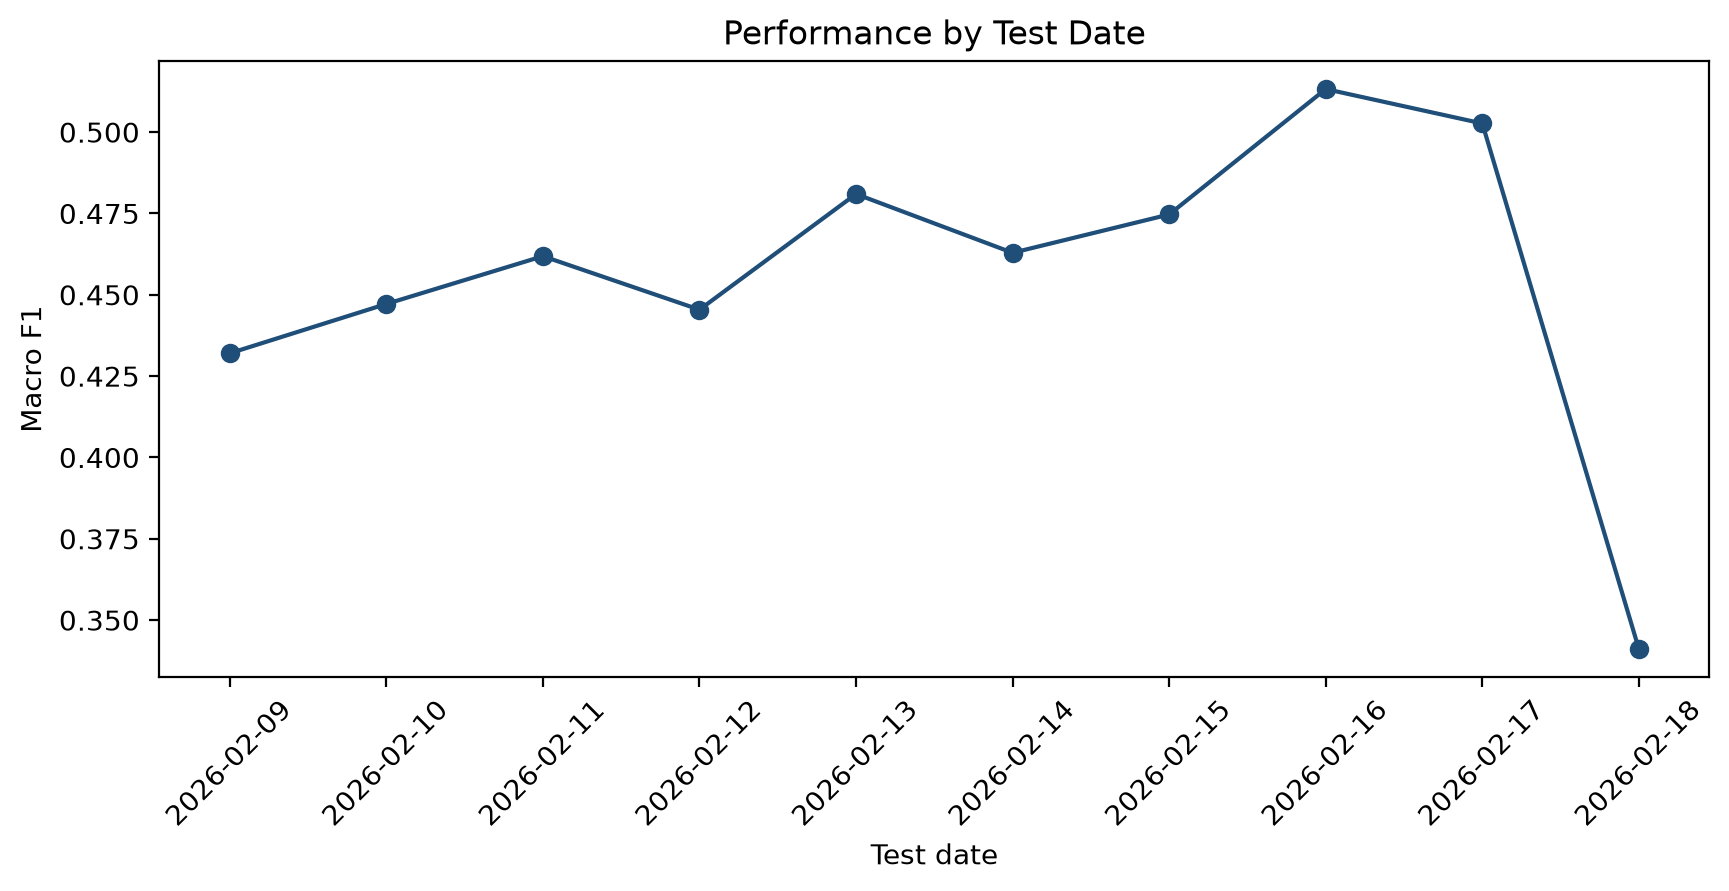
\includegraphics[width=\linewidth]{figures/models/performance_by_date.png}
\caption*{Performance by date}
\end{subfigure}
\hfill
\begin{subfigure}[t]{0.47\linewidth}
\centering

\includegraphics[width=\linewidth]{figures/models/performance_by_hour.png}
\caption*{Performance by hour}
\end{subfigure}
\end{figure}

\subsection{Feature-set comparison}

\begin{center}
\begin{tabular}{L{0.22\linewidth}L{0.22\linewidth}L{0.22\linewidth}L{0.22\linewidth}}
\toprule
Experiment & \#feats & Val Macro F1 & Test Macro F1 \\
\midrule
price\_only & 12 & 0.367 & 0.417 \\
static\_lob & 34 & 0.376 & 0.404 \\
dynamic\_lob & 30 & 0.349 & 0.420 \\
lob\_full & 64 & 0.374 & 0.456 \\
\textbf{full\_no\_trade} & \textbf{80} & \textbf{0.384} & \textbf{0.464} \\
full\_with\_trade & 89 & 0.397 & 0.463 \\
full\_no\_time & 76 & 0.379 & 0.459 \\
\bottomrule
\end{tabular}
\end{center}
\vspace{0.35em}

\begin{figure}[H]
\centering
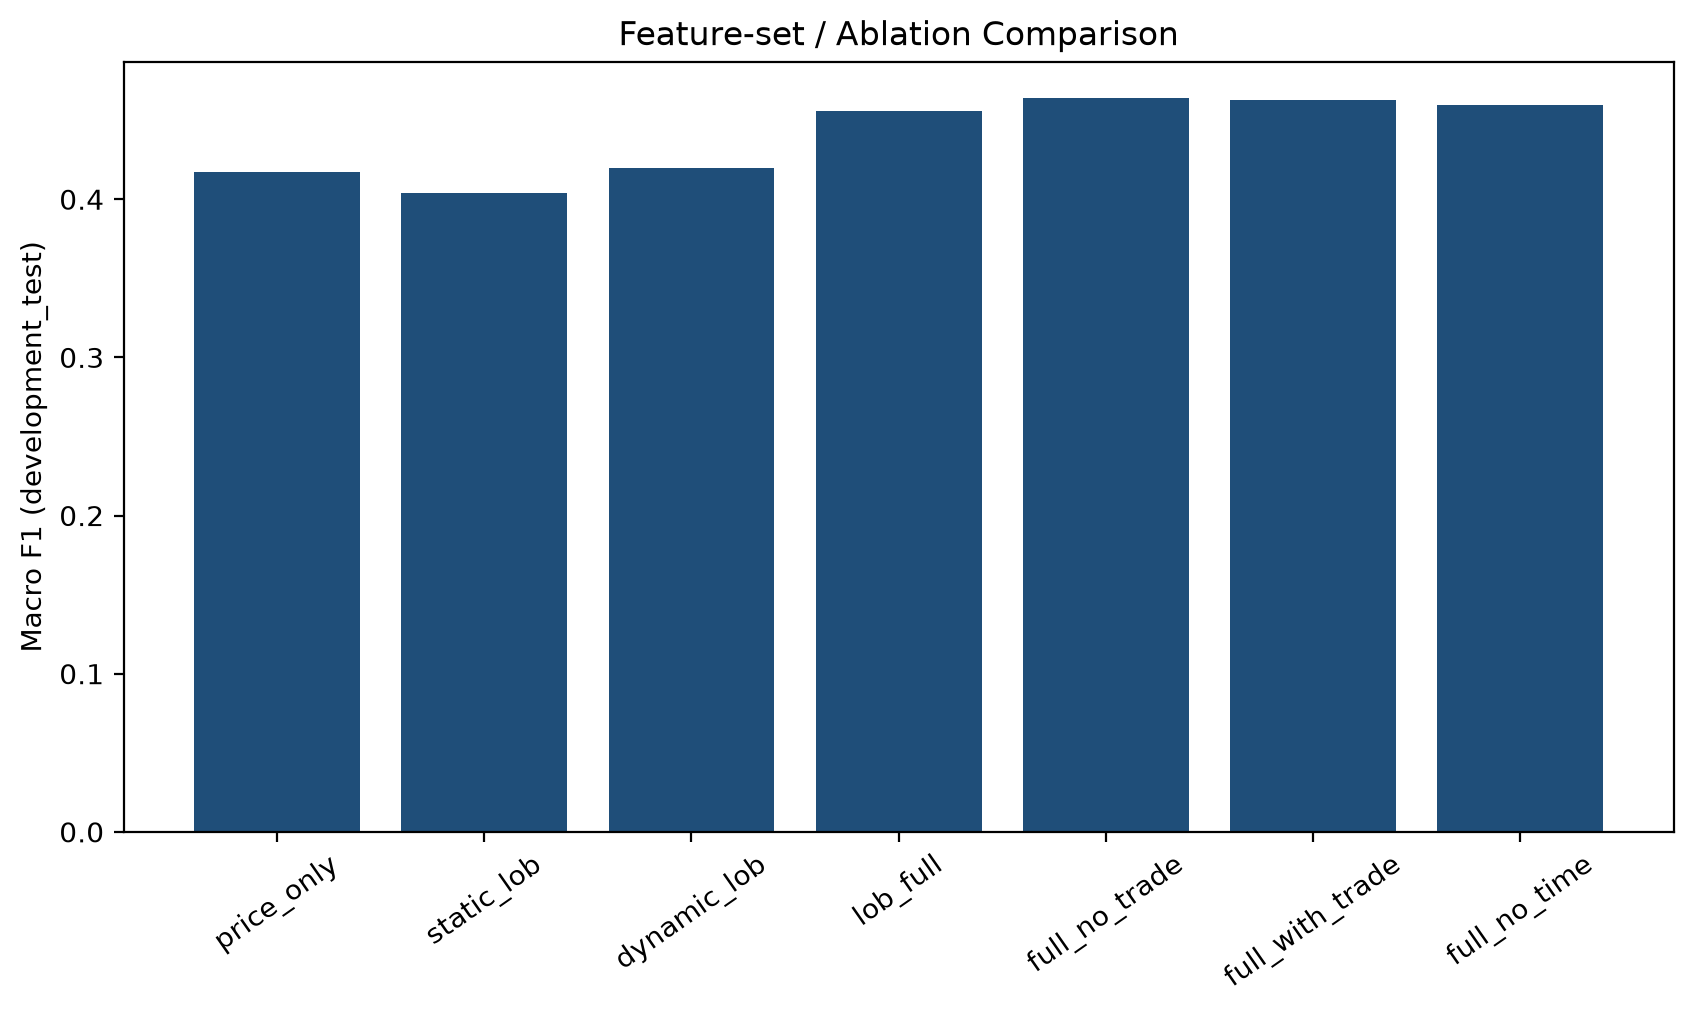
\includegraphics[width=0.80\linewidth]{figures/ablation/feature_set_comparison.png}
\caption{Feature set comparison}
\end{figure}

\begin{center}\textit{LOB features lift Macro F1 over price-only; corrected trades add essentially nothing.}\end{center}

\subsection{Study B}

Binary next-change direction Macro F1 $\approx$ \textbf{0.614} on development\_test (val $\approx$ 0.616). Easier task (no STABLE class; nearly balanced UP/DOWN).


\subsection{Study C}

Honest outcome: \textbf{10s/30s impossible} under observed gaps; \textbf{60s} has many eligible rows historically concentrated before the sparse test regime, so purged development\_test is empty $\rightarrow$ pilot descriptive stats only.


\subsection{Financial sanity (exploratory --- not a strategy)}

Long-only if predict UP (next mid return as proxy):


\begin{center}
\begin{tabular}{L{0.28\linewidth}L{0.28\linewidth}L{0.28\linewidth}}
\toprule
Scenario & Fees+slip (bps) & Mean net (bps) \\
\midrule
Zero cost & 0 & +0.92 \\
Low cost & 10 & \textbf{-2.35} \\
Moderate cost & 25 & \textbf{-7.25} \\
\bottomrule
\end{tabular}
\end{center}
\vspace{0.35em}

\begin{quote}
Sparse snapshots \textbf{do not} support a realistic HFT execution backtest. Prediction $\ne$ profitability.
\end{quote}

\vspace{0.5em}

\section{14. Explainability}

We require \textbf{agreement} across methods before calling a feature ``strongly supported''. SHAP answers \textit{how the trained model uses features for a prediction}, \textbf{not} whether a feature causes the mid-price to move in the market.


\subsection{How to read this section}

\begin{center}
\begin{tabular}{L{0.28\linewidth}L{0.28\linewidth}L{0.28\linewidth}}
\toprule
Plot / table category & What it answers & What it does \textit{not} say \\
\midrule
\textbf{Global importance bar} & Which features move predictions the most \textit{on average} & Direction of effect; causality \\
\textbf{Feature families} & Which microstructure \textit{families} dominate attributions & That every member of the family is useful \\
\textbf{Permutation importance} & Which features hurt Macro F1 when shuffled on held-out data & Local story for one snapshot \\
\textbf{Beeswarm (per class)} & Full distribution of attributions for DOWN / STABLE / UP & A single ``typical'' row \\
\textbf{Dependence} & How SHAP for feature $X$ changes as $X$ varies (often colored by a second feature) & Pure partial effect free of collinearity \\
\textbf{Local waterfalls} & Step-by-step attribution for one illustrative prediction & Population-level ranking \\
\textbf{Interactions} & Whether features co-contribute in TreeSHAP (or dependence fallbacks) & Causal interaction in the market \\
\bottomrule
\end{tabular}
\end{center}
\vspace{0.35em}

\subsection{Top TreeSHAP features (Study A)}

\textbf{What this table / bar chart says:} mean absolute SHAP over the development-test SHAP sample. Larger mean \textbackslash{}|SHAP\textbackslash{}| $\Rightarrow$ the feature tends to push the model's class scores more strongly across snapshots. Rankings are class-averaged for the 3-class model.


\begin{center}
\begin{tabular}{L{0.16\linewidth}L{0.16\linewidth}L{0.16\linewidth}L{0.16\linewidth}L{0.16\linewidth}L{0.16\linewidth}}
\toprule
Rank & Feature & Mean \textbackslash{} & SHAP\textbackslash{} &  & Family \\
\midrule
1 & \texttt{bid\_distance\_3\_bps} & 0.0595 & Static imbalance &  &  \\
2 & \texttt{ask\_distance\_2\_bps} & 0.0454 & Static imbalance &  &  \\
3 & \texttt{ask\_distance\_3\_bps} & 0.0345 & Static imbalance &  &  \\
4 & \texttt{volatility\_120s} & 0.0316 & Volatility &  &  \\
5 & \texttt{volatility\_300s} & 0.0304 & Volatility &  &  \\
6 & \texttt{bid\_distance\_2\_bps} & 0.0304 & Static imbalance &  &  \\
7 & \texttt{spread\_std\_300s} & 0.0203 & Dynamic liquidity &  &  \\
8 & \texttt{log\_ask\_depth\_1} & 0.0191 & Static depth &  &  \\
9 & \texttt{obi\_1} & 0.0179 & Static imbalance &  &  \\
10 & \texttt{hour\_cos} & 0.0163 & Time &  &  \\
\bottomrule
\end{tabular}
\end{center}
\vspace{0.35em}

\begin{figure}[H]
\centering

\includegraphics[width=0.80\linewidth]{figures/shap/shap_global_importance.png}
\caption{Global SHAP importance}
\end{figure}

\begin{center}\textit{Global bar plot --- average magnitude of attribution; does not encode sign (UP vs DOWN).}\end{center}

\subsection{Top feature families (sum of mean \textbackslash{}|SHAP\textbackslash{}|)}

\textbf{What this says:} we sum mean \textbackslash{}|SHAP\textbackslash{}| within each engineered family (static imbalance, volatility, depth, ...). It answers \textit{which family of LOB ideas the model leans on}, not which single column is ``best.''


\begin{enumerate}
\item \textbf{Static imbalance}  
\item Volatility  
\item Static depth  
\item Snapshot OFI proxy  
\item Static liquidity  
\end{enumerate}

\subsection{Permutation importance (top)}

\textbf{What this says:} features are randomly shuffled within the development-test set (respecting day blocks where configured); the drop in Macro F1 measures \textit{predictive usefulness under the evaluation metric}. Agreement with TreeSHAP is stronger evidence than either method alone.


\begin{enumerate}
\item \texttt{bid\_distance\_3\_bps}  
\item \texttt{ask\_distance\_2\_bps}  
\item \texttt{relative\_spread\_bps}  
\item \texttt{ask\_distance\_3\_bps}  
\item \texttt{hour\_cos}  
\end{enumerate}

Distance / imbalance features appear in \textbf{both} SHAP and permutation --- stronger evidence than \texttt{hour\_cos} alone.


\subsection{Beeswarm plots (class-conditional)}

\textbf{What beeswarm plots say:} for each class (DOWN / STABLE / UP), every point is one snapshot.

\begin{itemize}
\item \textbf{Vertical axis:} features ranked by mean \textbackslash{}|SHAP\textbackslash{}| for that class  
\item \textbf{Horizontal axis:} SHAP value (left = pushes \textit{against} that class; right = pushes \textit{for} it)  
\item \textbf{Color:} raw feature value (typically blue = low, red = high)
\end{itemize}

Use them to see \textit{patterns}: e.g. high imbalance features clustering on the positive side for UP, or volatility spreading attributions for STABLE. Because Study A is multiclass, we plot \textbf{one beeswarm per class} so attributions are not mixed across DOWN/STABLE/UP.


\begin{figure}[H]
\centering
\begin{subfigure}[t]{0.32\linewidth}
\centering

\includegraphics[width=\linewidth]{figures/shap/shap_beeswarm_down.png}
\caption*{DOWN}
\end{subfigure}
\hfill
\begin{subfigure}[t]{0.32\linewidth}
\centering

\includegraphics[width=\linewidth]{figures/shap/shap_beeswarm_stable.png}
\caption*{STABLE}
\end{subfigure}
\hfill
\begin{subfigure}[t]{0.32\linewidth}
\centering

\includegraphics[width=\linewidth]{figures/shap/shap_beeswarm_up.png}
\caption*{UP}
\end{subfigure}
\end{figure}

\begin{center}\textit{Class-conditional beeswarms --- distribution of attributions, not a single summary number.}\end{center}

\subsection{Dependence plots}

\textbf{What dependence plots say:} for a chosen feature $X$, each point is a snapshot plotted as $(X,\ \mathrm{SHAP}_X)$ for the \textbf{UP} class contribution (when multiclass). Color usually marks an automatically chosen interacting feature. They reveal \textit{how} the model's attribution changes as $X$ moves (nonlinear / threshold behavior) and hint at pairwise co-dependence.


They do \textbf{not} isolate a causal partial effect: correlated LOB features can share credit.


\begin{figure}[H]
\centering
\begin{subfigure}[t]{0.47\linewidth}
\centering

\includegraphics[width=\linewidth]{figures/shap/shap_dependence_obi_5.png}
\caption*{OBI (depth 5)}
\end{subfigure}
\hfill
\begin{subfigure}[t]{0.47\linewidth}
\centering

\includegraphics[width=\linewidth]{figures/shap/shap_dependence_weighted_obi.png}
\caption*{Weighted OBI}
\end{subfigure}
\end{figure}

\begin{figure}[H]
\centering
\begin{subfigure}[t]{0.47\linewidth}
\centering

\includegraphics[width=\linewidth]{figures/shap/shap_dependence_relative_spread_bps.png}
\caption*{Relative spread}
\end{subfigure}
\hfill
\begin{subfigure}[t]{0.47\linewidth}
\centering

\includegraphics[width=\linewidth]{figures/shap/shap_dependence_microprice_edge_bps.png}
\caption*{Microprice edge}
\end{subfigure}
\end{figure}

\begin{figure}[H]
\centering
\begin{subfigure}[t]{0.47\linewidth}
\centering
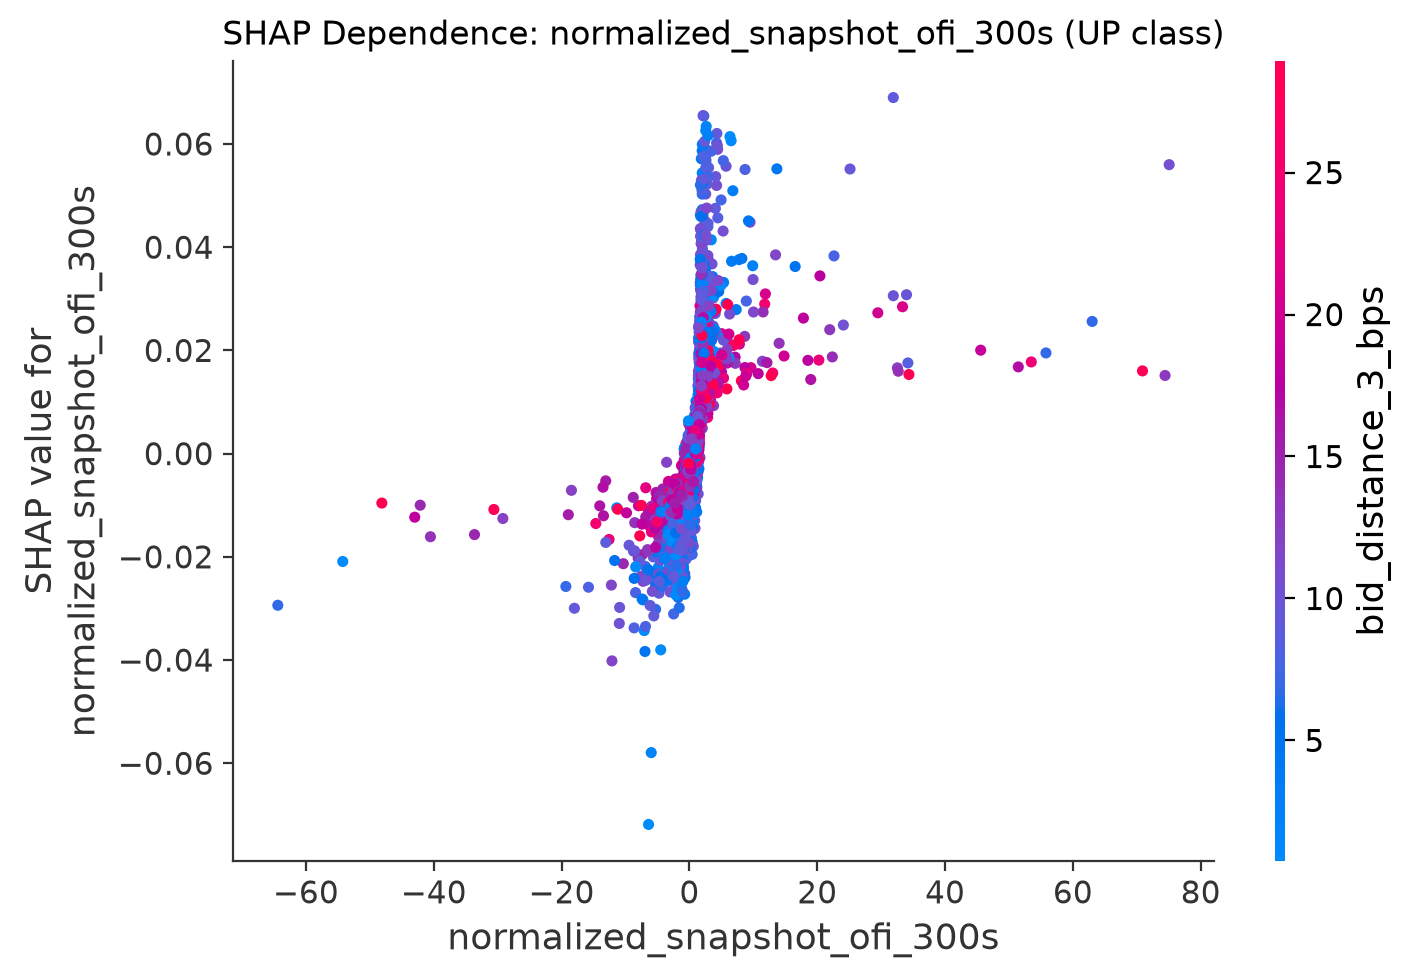
\includegraphics[width=\linewidth]{figures/shap/shap_dependence_normalized_snapshot_ofi_300s.png}
\caption*{Normalized snapshot OFI (300s)}
\end{subfigure}
\hfill
\begin{subfigure}[t]{0.47\linewidth}
\centering

\includegraphics[width=\linewidth]{figures/shap/shap_dependence_volatility_300s.png}
\caption*{Volatility (300s)}
\end{subfigure}
\end{figure}

\begin{center}\textit{Dependence plots --- functional shape of attribution vs feature value (UP-class SHAP).}\end{center}

\subsection{Local waterfalls (illustrative cases)}

\textbf{What waterfall plots say:} for \textbf{one} snapshot, starting from the model's expected score (base value), each bar shows how a feature pushes the score up or down until the final prediction for the highlighted class. They are case studies, not rankings.


We pick five illustrative development-test cases:


\begin{center}
\begin{tabular}{L{0.32\linewidth}L{0.58\linewidth}}
\toprule
Case & What it is meant to show \\
\midrule
\textbf{Correct high-conf UP} & Confident correct UP --- which LOB features drove the UP score \\
\textbf{Correct high-conf DOWN} & Same for DOWN \\
\textbf{Correct high-conf STABLE} & Same for STABLE (often spread / low-move cues) \\
\textbf{Incorrect high-conf} & Confident but wrong --- where the model ``trusted'' misleading features \\
\textbf{Low-conf borderline} & Near-tie probabilities --- small opposing attributions \\
\bottomrule
\end{tabular}
\end{center}
\vspace{0.35em}

\begin{figure}[H]
\centering
\begin{subfigure}[t]{0.47\linewidth}
\centering

\includegraphics[width=\linewidth]{figures/shap/shap_waterfall_correct_high_conf_UP.png}
\caption*{Correct high-conf UP}
\end{subfigure}
\hfill
\begin{subfigure}[t]{0.47\linewidth}
\centering

\includegraphics[width=\linewidth]{figures/shap/shap_waterfall_correct_high_conf_DOWN.png}
\caption*{Correct high-conf DOWN}
\end{subfigure}
\end{figure}

\begin{figure}[H]
\centering
\begin{subfigure}[t]{0.47\linewidth}
\centering

\includegraphics[width=\linewidth]{figures/shap/shap_waterfall_correct_high_conf_STABLE.png}
\caption*{Correct high-conf STABLE}
\end{subfigure}
\hfill
\begin{subfigure}[t]{0.47\linewidth}
\centering

\includegraphics[width=\linewidth]{figures/shap/shap_waterfall_incorrect_high_conf.png}
\caption*{Incorrect high-conf}
\end{subfigure}
\end{figure}

\begin{figure}[H]
\centering

\includegraphics[width=0.70\linewidth]{figures/shap/shap_waterfall_low_conf_borderline.png}
\caption{Waterfall borderline}
\end{figure}

\begin{center}\textit{Local waterfalls --- per-snapshot accounting of the model's score; not causal market effects.}\end{center}

\subsection{SHAP interactions}

\textbf{What this category says:} TreeSHAP can estimate pairwise \textit{interaction values} (extra attribution when two features act together beyond main effects). We reduce the multiclass tensor to a 2-D mean-absolute interaction matrix when possible and save \texttt{reports/tables/shap\_interactions\_native.csv}. If that fails, we log the failure and fall back to colored dependence plots under \texttt{reports/figures/shap/} --- \textbf{never} fabricated interaction numbers.


\textbf{Latest run status:} see \texttt{reports/metrics/shap\_interaction\_status.json}.


Regenerate without full retuning: \texttt{python scripts/regenerate\_shap\_plots.py}


\vspace{0.5em}

\section{15. Challenges we hit}

This section is intentional --- sharing failures is what makes the project credible.


\begin{center}
\begin{tabular}{L{0.28\linewidth}L{0.28\linewidth}L{0.28\linewidth}}
\toprule
Challenge & What happened & Resolution \\
\midrule
\textbf{Misleading fixed horizons} & 10/30/60s often mapped to the \textit{same} next snapshot & Redesign into Studies A/B/C; store actual delays \\
\textbf{Sparse gaps} & Median \textasciitilde{}69s; test \textasciitilde{}189s; 100\% of gaps > 60s & No 5s forward-fill; longer feature windows (120--1200s) \\
\textbf{Study C empty horizons} & 0 eligible rows for 10s \& 30s & Label as underpowered pilot; do not invent scores \\
\textbf{Study C 60s purge} & Eligible overall, but development\_test left with 0 after target purge & Descriptive-only; no robust model claim \\
\textbf{Repeated last trades} & Same \texttt{last\_trade\_*} across many snapshots & \texttt{trade\_deduplication.py}; exclude from primary \\
\textbf{Tiny tick in bps} & Tick=10 IRT $\rightarrow$ \textasciitilde{}1e-6 bps vs huge mid & Hybrid $\varepsilon$ uses quantiles/spreads \\
\textbf{CatBoost API} & \texttt{bagging\_temperature} invalid with Bernoulli bootstrap & Dropped temperature; keep Bernoulli + subsample \\
\textbf{SHAP interactions} & Multiclass tensor needs careful 2-D reduction & Reduce over samples/classes or use dependence fallbacks \\
\textbf{macOS XGBoost} & Needs \texttt{libomp} & \texttt{.libs/libomp.dylib} + \texttt{DYLD\_LIBRARY\_PATH} in scripts \\
\textbf{Development-test contamination} & Prior analysis already looked at late dates & Renamed; require future holdout \\
\textbf{Class imbalance} & STABLE dominates under hybrid $\varepsilon$ & Macro F1 primary; balanced sample weights \\
\bottomrule
\end{tabular}
\end{center}
\vspace{0.35em}

Archived v1 metrics live in \texttt{reports/archive/pre\_research\_redesign/} and must \textbf{not} be mixed with v2 claims.


\vspace{0.5em}

\section{16. What we do \textit{not} claim}

\begin{itemize}
\item True high-frequency forecasting from these sparse snapshots  
\item Exact 30-second prediction when the next print is minutes away  
\item Causal effects from SHAP  
\item Trading profitability / production alpha  
\item True event-level OFI  
\item Generalization to all crypto markets  
\item That CatBoost ``wins'' without multi-fold statistical comparison  
\item That the development\_test is a final holdout  
\end{itemize}

\vspace{0.5em}

\section{17. Reproduction}

\begin{verbatim}
git clone git@github.com:OveysSayad/explainable-btcirt-lob.git
cd explainable-btcirt-lob

python -m venv .venv
source .venv/bin/activate
pip install -r requirements.txt
pip install -e .

# Place the raw CSV:
#   data/raw/market_data_clean_nobitex.csv

# macOS XGBoost OpenMP:
#   brew install libomp
#   mkdir -p .libs && ln -sf "$(brew --prefix libomp)/lib/libomp.dylib" .libs/libomp.dylib
export DYLD_LIBRARY_PATH="$(pwd)/.libs:${DYLD_LIBRARY_PATH}"

./scripts/run_pipeline.sh
pytest -q
\end{verbatim}

Makefile targets: \texttt{make test}, \texttt{make all}, \texttt{make study-a}, \texttt{make study-b}, \texttt{make study-c}.


Smoke (fewer trials): \texttt{python -m src.pipeline --config configs/smoke\_config.yaml}.


\vspace{0.5em}

\section{18. Outputs catalog}

\begin{center}
\begin{tabular}{L{0.32\linewidth}L{0.58\linewidth}}
\toprule
Path & Contents \\
\midrule
\texttt{reports/final\_report.md} & Paper-style write-up \\
\texttt{reports/tables/*.csv} & Metrics, gaps, SHAP, ablations, predictions metadata \\
\texttt{reports/ARTIFACT\_MANIFEST.md} & Canonical vs archive artifact map \\
\texttt{reports/metrics/*.json} & Environment, bootstrap, study metrics, interaction status \\
\texttt{reports/figures/} & Data quality, labels, models, SHAP, ablation (embedded in this README) \\
\texttt{reports/models/frozen\_model\_specification.json} & Frozen Study A spec \\
\texttt{models/study\_a/}, \texttt{models/study\_b/} & Trained model artifacts \\
\bottomrule
\end{tabular}
\end{center}
\vspace{0.35em}

Figure layout:


\begin{verbatim}
reports/figures/
├── data_quality/   # gaps, mid, spread, depth, coverage
├── labels/         # class mix, returns vs ε, OBI
├── models/         # comparison, confusion, ROC/PR, calibration
├── shap/           # beeswarm, dependence, waterfalls
├── ablation/       # feature-set comparison
└── robustness/     # reserved
\end{verbatim}
| \texttt{reports/archive/pre\_research\_redesign/} | Pre-redesign freeze |

| \texttt{docs/} | Design, formulas, validation, dense-collection plan |


\vspace{0.5em}

\section{19. Limitations \& future work}

See \href{docs/LIMITATIONS.md}{\texttt{docs/LIMITATIONS.md}}.


\textbf{Highest-priority next steps}


\begin{enumerate}
\item Collect \textbf{dense} WebSocket LOB + trades (\texttt{docs/DENSE\_DATA\_COLLECTION\_DESIGN.md})  
\item Evaluate the \textbf{frozen} model on \textbf{$\ge$7--14 new days} never used in analysis  
\item Complete nested walk-forward \textit{scores} (fold Macro F1 distribution), not only fold calendars  
\item Stronger time-feature artifact tests (gap/hour confounds)
\end{enumerate}

\vspace{0.5em}

\section{20. Research integrity}

\begin{itemize}
\item No fabricated metrics, figures, API responses, or SHAP interactions  
\item Failed / underpowered components remain documented  
\item Prior results archived, not silently overwritten without copy  
\item Primary metric Macro F1 chosen for class imbalance --- not to hide weak DOWN/UP performance  
\item \textbf{Final independent holdout evaluation pending}
\end{itemize}

\vspace{0.5em}

\section{Citation}

\begin{verbatim}
@software{explainable_btcirt_lob,
  title  = {Explainable ML for BTCIRT Limit Order Book Dynamics},
  author = {Sayad, Oveys},
  year   = {2026},
  url    = {https://github.com/OveysSayad/explainable-btcirt-lob},
  note   = {Multi-study redesign under sparse Nobitex snapshots}
}
\end{verbatim}

\section{Disclaimer}

Research and education only. \textbf{Not investment advice.} Cryptocurrency trading involves substantial risk of loss.


\vspace{0.5em}

\subsection{Bottom line for readers \& recruiters}

This repo demonstrates \textbf{research engineering}: questioning a bad horizon design, quantifying sparsity, preventing leakage, comparing models fairly, and explaining predictions without overselling. That is rarer --- and more valuable --- than another notebook that reports a high F1 on shuffled LOB rows.


\end{document}
